%% The following is a directive for TeXShop to indicate the main file
%%!TEX root = ../diss.tex

\chapter{Oxygen enhanced MRI - Validation of method in animals}
\label{ch:oemri2}

% ======================================================================
\section{Introduction}
% ======================================================================

Dynamic oxygen enhanced MRI (dOE-MRI) has recently been proposed by our group to assess tumour oxygenation in vivo using MRI~\cite{Moosvi:2018ca}.
In this chapter we first validate the method in tumour xenografts and compare dOE-MRI maps to slice-matched histological sections.
Next we present a model that phenomenologically describes the kinetics of the oxygen response in tumours. 
This model is then fit to the extracted ICA components from all imaged animals to assess the feasibility of using the fit parameters as biomarkers of oxygen response.

\subsection{Theory: Modelling oxygen response}
\label{sec:lognormalfitting_theory}
A vascular network is a collection of multiple vessels including large arteries feeding smaller arterioles that ultimately deliver oxygen and nutrients to tissue via capillaries.
This complex vascular tree is modelled by assuming a fractal branching geometry with the distribution of vessel sizes and flow rates given by a lognormal velocity distribution~\cite{Qian:2000ca}:

\begin{equation}
P(v)=\frac{1}{\sigma_{f} \sqrt{2 \pi}} \cdot \frac{1}{v} \cdot \exp \left(-\frac{1}{2}\left(\frac{\ln (v)-u_{f}}{\sigma_{f}}\right)^{2}\right)
\end{equation}

Where $P(v)$ is the probability density function of the velocity $v$, $\mu_f$ and $\sigma_f$ are the mean and standard deviation of the distribution for the normally distributed random variable $ln(v)$.
The mean of a lognormal distribution are known quantities,

\begin{equation}
\operatorname{Mean}(v)=\exp \left(\mu_{f}+\frac{\sigma_{f}^{2}}{2}\right)
\end{equation}

\begin{equation}
\operatorname{Var}(v)=\exp \left(2 \mu_{f}+\sigma_{f}^{2}\right)\cdot \left(\exp \left(\sigma_{f}^{2}\right)-1\right)
\end{equation}

\begin{figure}[htbp]
   \centering
   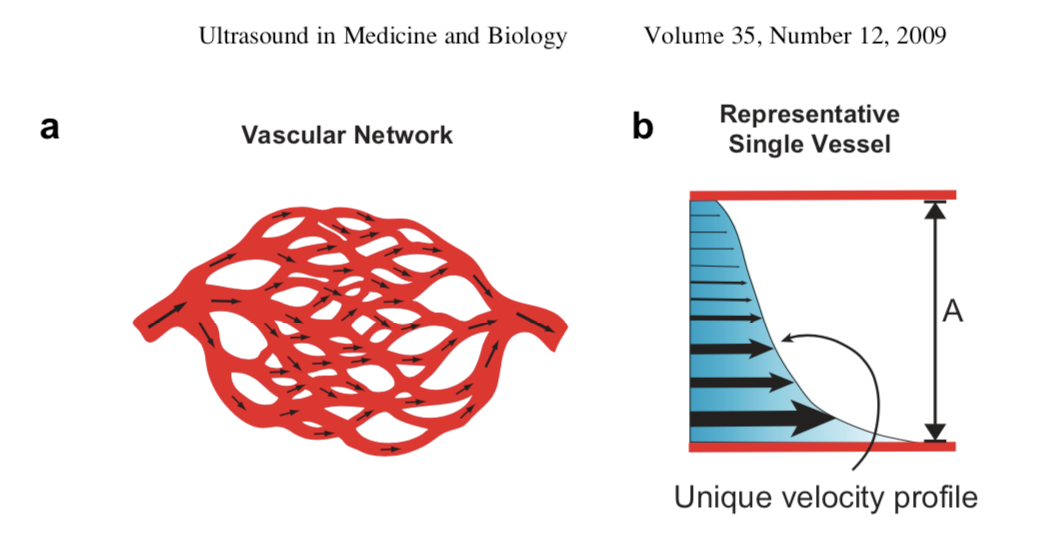
\includegraphics[width=\textwidth]{oemri_thesis2/oemri_thesis2-images/lognormal.png} % requires the graphicx package
   \caption{Schematic representation of the complex vascular network modelled as a representative single vessel with multiple flow profiles, from Hudson et al 2009~\cite{Hudson:2009jv}. The distribution of velocity profiles of the representative single vessel is the lognormal distribution.}
   \label{lognormal}
\end{figure}

Figure~\ref{lognormal} shows a schematic of the vascular network modelled as a representative single vessel with a lognormal distribution of velocity profiles~\todo{Need to adapt and re-create or ask for permission to re-use?}.
Therefore the flow function for a vascular network is given by,

\begin{equation}
F(z, t)=\frac{A}{2} \cdot \operatorname{erfc}\left(\frac{\ln (z / t)-u_{f}}{\sigma_{f} \sqrt{2}}\right)
\end{equation}

Where A is defined as the total vascular area, z represents the spatial displacement of oxygen through the blood stream, $\mu_f$ is the mean velocity and $\sigma_f$ is the standard deviation of the velocity distributions. 
The velocity $v$ has been transformed to $z/t$ for convenience and ease of interpretation.

This lognormal flow profile model has been used to describe the replenishment of microbubbles injected into the blood stream in dynamic contrast enhanced ultrasound (DCE-US)~\cite{Hudson:2009jv}.
The generalized representation of the replenishment time-intensity signal requires two components: an ultrasound beam-specific profile that is weighted in the z-direction due to a non-uniform slice profile and the flow profile. 
The expression is,

\begin{equation}
S(t) = \int_{V} B(x,y,z) \cdot F(x,y,z,t) \cdot dV
\end{equation}

where $B(x,y,z) = 1$ in MRI because of relatively uniform slice profiles. 
Integrating over the imaging plane (x,y) and assuming a slice thickness of 1mm (z), the final model for fitting dOE-MRI data becomes,

\begin{equation}
S(t)= \left[\frac{A}{2}\left(z \operatorname{erfc}\left(\frac{\ln \left(z/t\right)-\mu_f}{\sqrt{2} \sigma_f}\right)-t e^{\sigma_f^{2} / 2+\mu_f} \operatorname{erf}\left(\frac{\sigma_f^{2}+\mu_f-\log \left(z/t\right)}{\sqrt{2} \sigma_f}\right)\right)\right]_{z=0}^{z=1mm}
\label{lognormalFitEquation}
\end{equation}

Where A is defined as the total vascular area, $\mu_f$ is the mean velocity and $\sigma_f$ is the standard deviation of the velocity distributions. 

% ======================================================================
\section{Methods}
% ======================================================================
\subsection{Animals}
Female NRG (NOD rag gamma) mice were implanted with murine squamous cell carcinoma (SCCVII; 5x10$^5$ cells in 50$\mu$l serum-free media; cells provided by Dr. J. Evans) in the dorsal subcutaneous region.
All mice were injected with 60 mg/kg pimonidazole hydrochloride (HypoxyProbe) 30 min prior to imaging to label hypoxic cells and were euthanized within 15 min of imaging completion.
Mice were anesthetized with isoflurane using 1.5-2.0\% isoflurane for the duration of MR imaging sessions until euthanasia, and were positioned supine on the custom surface coil apparatus.
Throughout the imaging session, a small animal monitoring system (SAII Instruments, Stony Brook, NY, USA) was used to monitor respiration rate, varying between 80-100 breaths per minute, and body temperature, maintained at 36.8 $\pm$ 0.5$^\circ$C using a continuous airflow heater. 
Tumours were embedded and frozen in optimum cutting temperature medium (OCT; Tissue-TEK) with their largest diameter 8-10 mm.
All animal experimental procedures were carried out in compliance with the guidelines of the Canadian Council for Animal Care and were approved by the institutional Animal Care Committee.

\subsection{Immunohistochemistry}
Co-planar MRI slices and histological sections were obtained by imaging perpendicular to the longest tumour axis in MRI and serial-step 10 $\mu m$ cryosections were cut at 0.5-mm intervals in the same plane.
Slides were then fixed in acetone-methanol for 10 min and whole sections were immunohistochemically stained~\cite{Kalra:2017is} for CD31 (PECAM; visualized using secondaries labeled with Alexa 647nm) to label blood vessels, and for pimonidazole (HypoxyProbe-1; visualized using secondary labeled with Alexa 546nm) to label hypoxic cells. Sections were then stained using Hoechst 33342 (bisbenzimide) to label all cell nuclei.
Whole-tumour sections were imaged using a robotic fluorescence microscope (Zeiss Axioimager Z1), a cooled, monochrome CCD camera (Retiga 4000R; QImaging), a motorized slide loader and x-y stage (Ludl Electronic Products) and customized ImageJ software~\cite{Collins:2007jr}. 
Adjacent microscope fields of view were tiled such that images of entire tumour cryosections were captured at a resolution of 1.5 $\mu m$/pixel. 
Using anatomical landmarks and accumulated thicknesses of serial-step sections as estimates of distances from the edges of whole tumours, sections were chosen to match the MR slices. 
ImageJ and user-supplied algorithms were used to super impose digital images which were then manually cropped to tumour tissue boundaries with staining artifacts removed. 
A threshold was applied to images to identify positive pimonidazole staining, and the number of positive pixels was determined as a percentage of the total number of pixels in the tumour image. 
Overlaid greyscale images were converted to false colour for visualization with pimonidazole as green and CD31 as magenta.

\subsection{MR Imaging}
As previously described in Section~\ref{doemri_mrianalysis1}.

\subsection{dOE-MRI Analysis}

As previously described in Section~\ref{doemri_mrianalysis2}.

\subsection{Model Fitting}
\label{sec:lognormalfitting_methods}
Equation~\ref{lognormalFitEquation} was fit to the first 100 seconds of the ICA component trace after oxygen was first delivered to the mouse. 
Model fitting was done with the \texttt{LMFIT} package~\cite{Newville:2014jt} using the Levenberg-Marquardt method.
A free fit parameter was added corresponding to a vertical offset to account for the ICA component starting below 0. 
For each fit, three parameters describe the shape of the oxygen response: A (vascular area), $\mu_f$ (mean velocity) and $\sigma_f$ (standard deviation) of the velocity distributions.
A sample fit using equation~\ref{lognormalFitEquation} is shown in figure~\ref{fig:lognormal_sample}.

\begin{figure}[htbp]
   \centering
   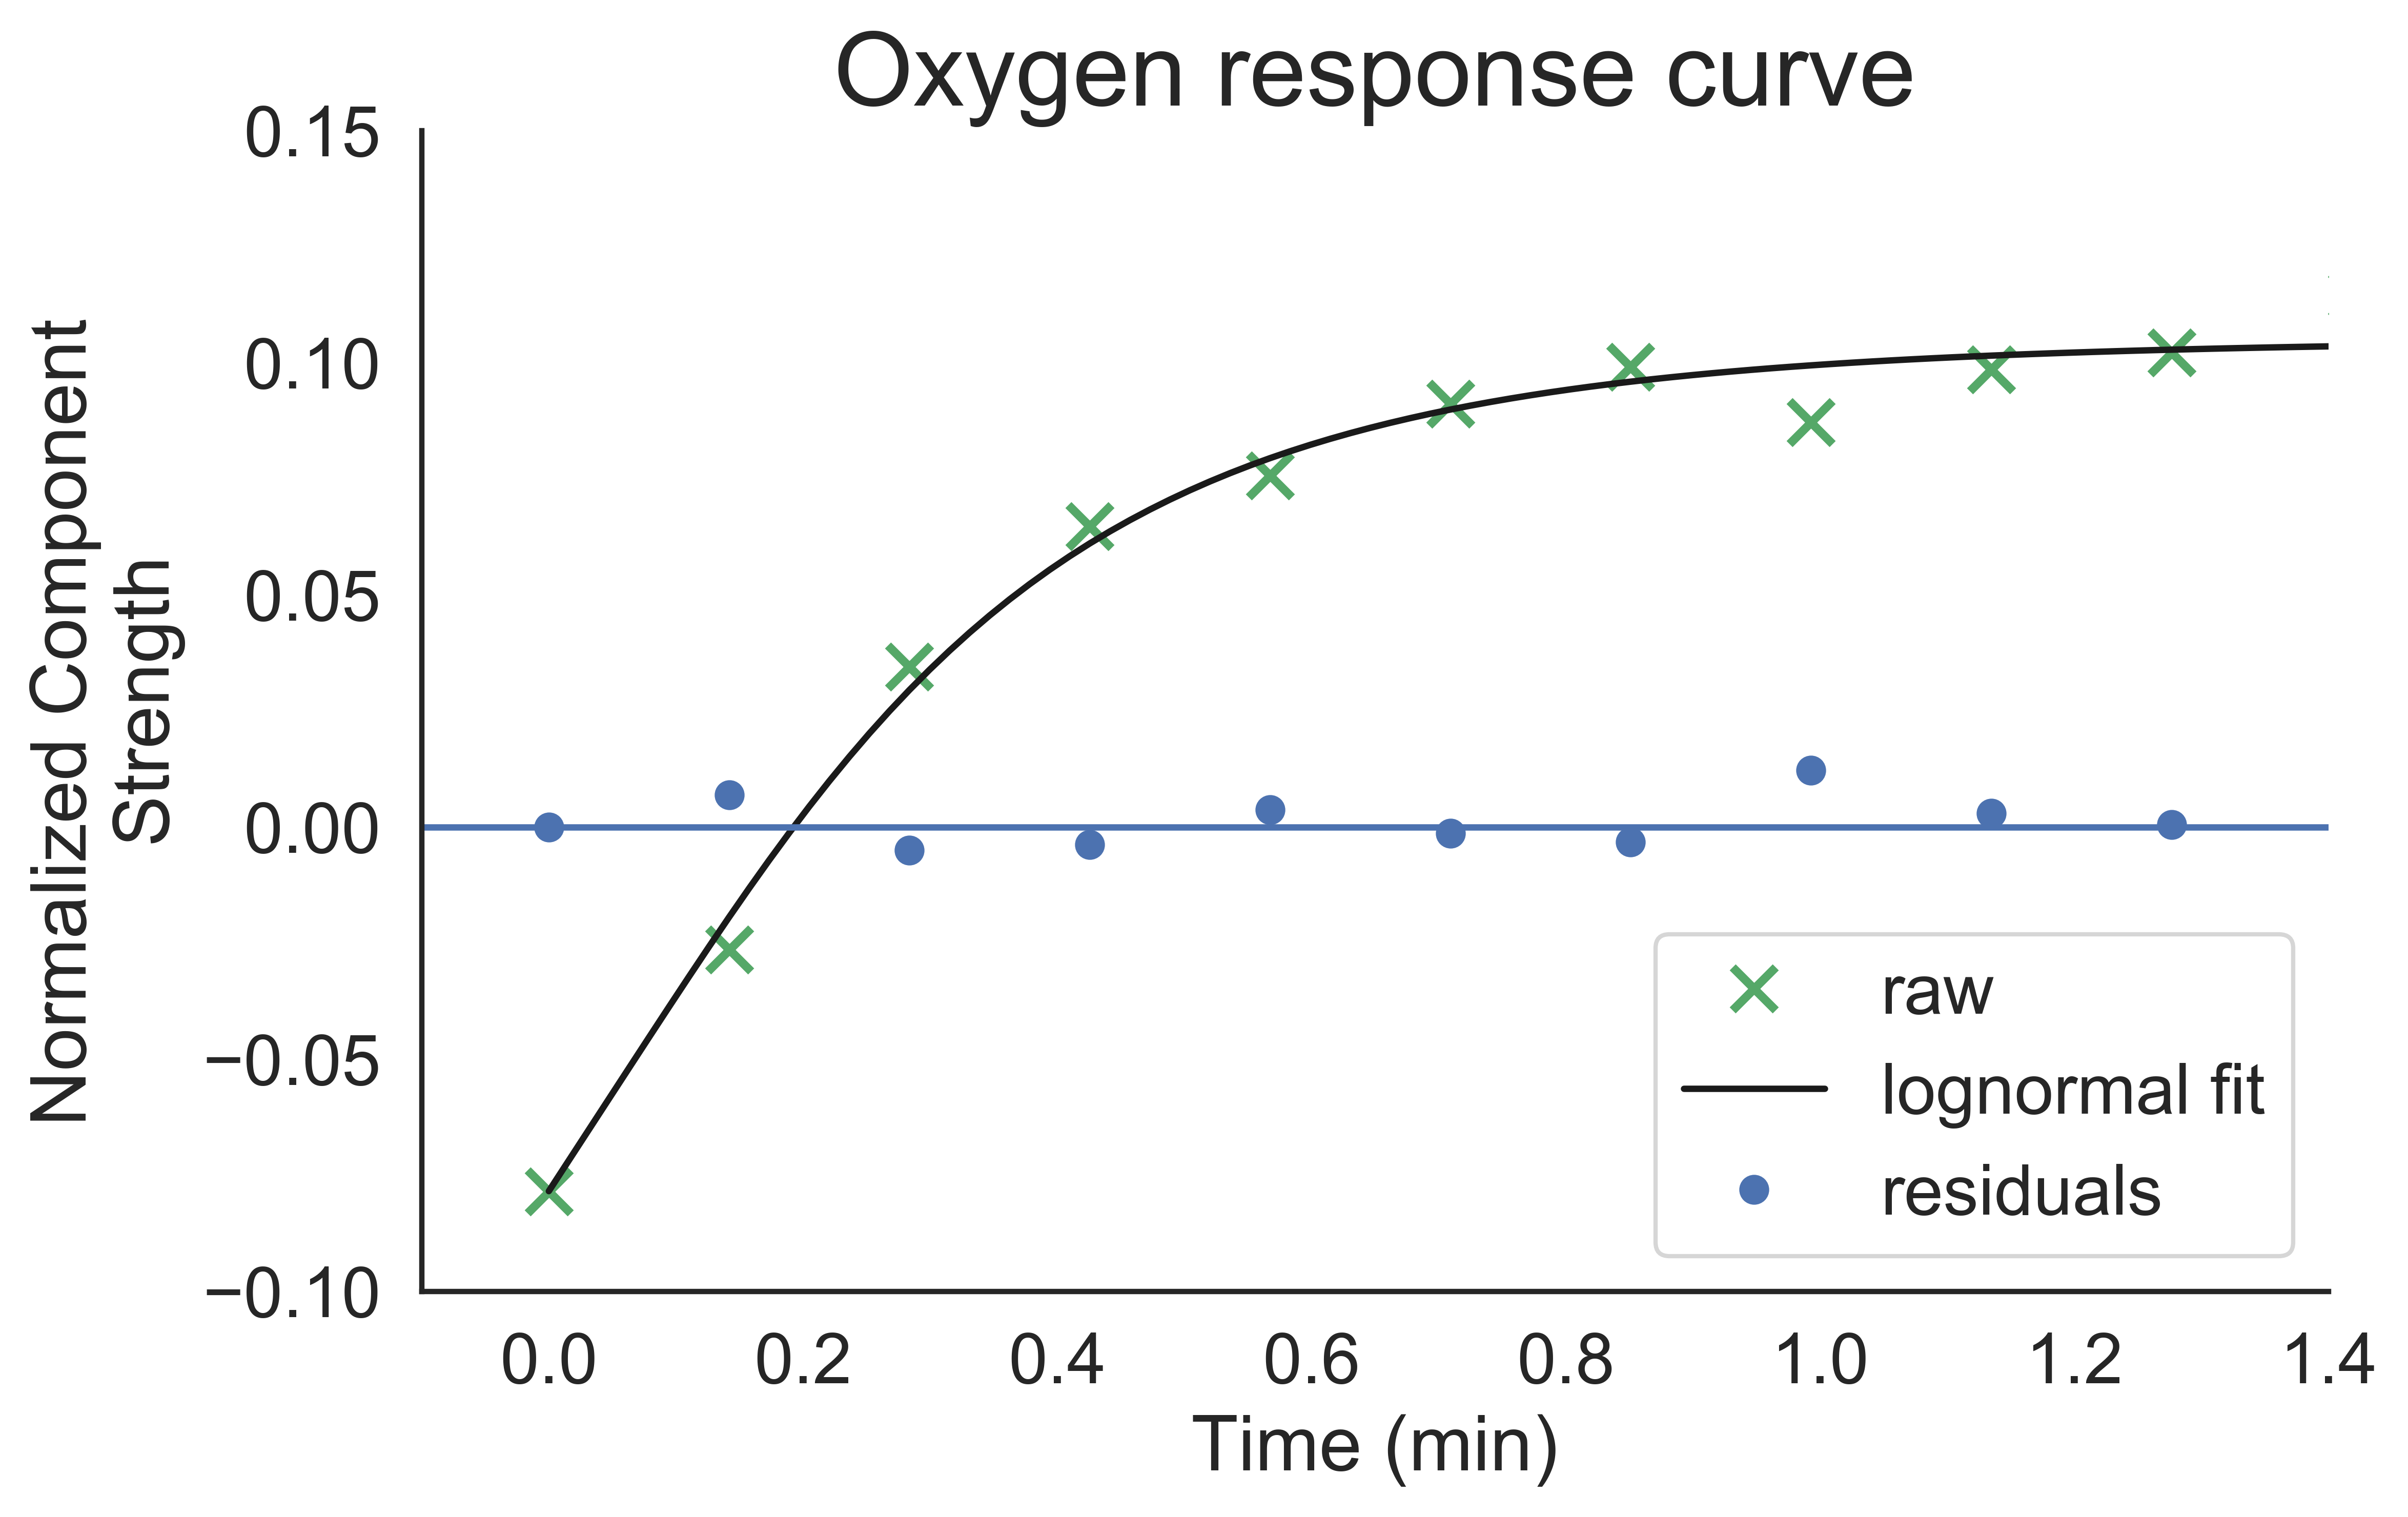
\includegraphics[width=\textwidth]{oemri_thesis2/oemri_thesis2-images/technical_SampleFit.png} % requires the graphicx package
   \caption{Fit of equation~\ref{lognormalFitEquation} to an oxygen response curve with the residuals plotted along the x-axis for each point.
   For this fit, $A= 0.18$, $v_f = 0.66 mm/s$, and $\sigma_f = 0.58 mm/s$.}
   \label{fig:lognormal_sample}
\end{figure}

% ======================================================================
\section{Results}
% ======================================================================
%%%%%%%%%%%%%%%%% ############ BEGIN *versatile* section from paper 1 ############ 
\subsection{ICA enabled dOE-MRI detects variable oxygenation in a range of tumour models}
\label{sec:rangeModels}
Tumours of human and murine origin and comprising a variety of tumour microenvironments were imaged, including fast growing, highly vascularized murine squamous cell (SCCVII) and human ovarian carcinomas (SKOV3), slower growing and well vascularized human breast cancer (BT-474), as well as a relatively fast growing but more poorly vascularized human colon colorectal carcinoma (HCT-116).
The inter-model heterogeneity of the tumours is reflected in the mean fraction of negative voxels in the dOE-MRI maps, which were 46 $\pm$ 6\% for BT-474, 36$\pm$3\% for HCT-116, 31$\pm$5\% for SCCVII, and 14$\pm$4\% for SKOV3 tumours. 
Considerable intra-tumour heterogeneity is also observed within some models, particularly the BT474.
dOE-MRI maps representing the mean fraction of negative voxels are shown for each tumour type in Figure~\ref{versatile}.
\begin{figure}[htbp]
   \centering
   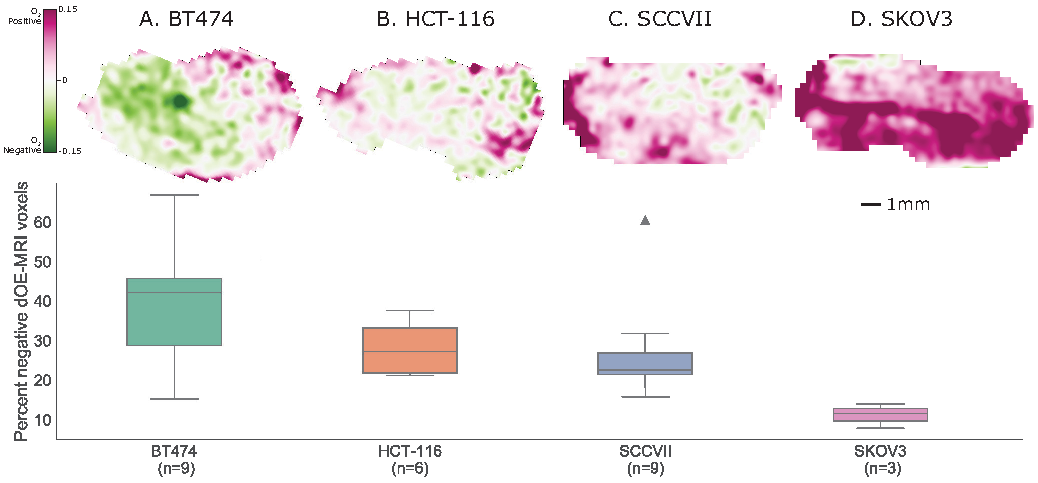
\includegraphics[width=\textwidth]{oemri_thesis1/oemri_thesis1-images/fig2_versatile.pdf} % requires the graphicx package
   \caption{Top: dOE-MRI maps for four tumour models HCT-116, BT-474, SCCVII, and SKOV3 are shown. Chosen slices are representative of the mean percent negative dOE-MRI fraction for the respective tumour model.
Bottom: The box-whisker plot shows the quartiles of percent negative dOE-MRI voxels for all imaged tumours.
\label{versatile}}
\end{figure}
%%%%%%%%%%%%%%%%% ############ END *versatile* section from paper 1########### 

%%%%%%%%%%%%%%%%% ############ BEGIN section about fitting ############

\subsection{Vascular area $A$ and mean velocity $v_f$ do not vary across tumour models, but $\sigma_f$ differentiates between tumours}
\label{sec:lognormalfitting_results}
% Analysis notebook: 
% http://localhost:8889/user/fmoosvi/notebooks/OxygenMRI/Thesis%20Exploring/OEMRI%20chapter%202%20-%20lognormal%20fitting%20aggregations.ipynb
Equation~\ref{lognormalFitEquation} was fit to the oxygen response kinetics for three tumour models (SCCVII, HCT-116, and BT474).
Figure~\ref{fig:lognormal_CHB} shows the raw data and the fit for each animal. 
Group averages for each of the three parameters $A$, $v_f$ and $\sigma_f$ are shown in box plots.
The parameter $\sigma_f$ discriminated between tumour types in this analysis and $\sigma_f$ for SCCVII tumours ($\sigma_f$ = 0.30 $\pm$ 0.09 mm/s) was statistically significantly lower than the HCT-116 tumours ($\sigma_f$ = 0.52 $\pm$ 0.12 mm/s; p = 0.047) as well as the BT474 tumours ($\sigma_f$ = 0.76 $\pm$ 0.19 mm/s; p = 0.044).
The effect size for both comparisons was quite small: Hedge's g = 0.05 for SCCVII vs. HCT-116 tumours and $g$ = 0.02 for SCCVII vs. BT474. 
No significant difference was found when comparing $\sigma_f$ of HCT-116 and BT474 tumours.
High intratumour variability was present in all tumours, but particularly in the BT474 tumour models.
The SKOV3 tumours were not considered as part of this analysis due to low sample size (N=3). 

\begin{figure}[htbp]
   \centering
   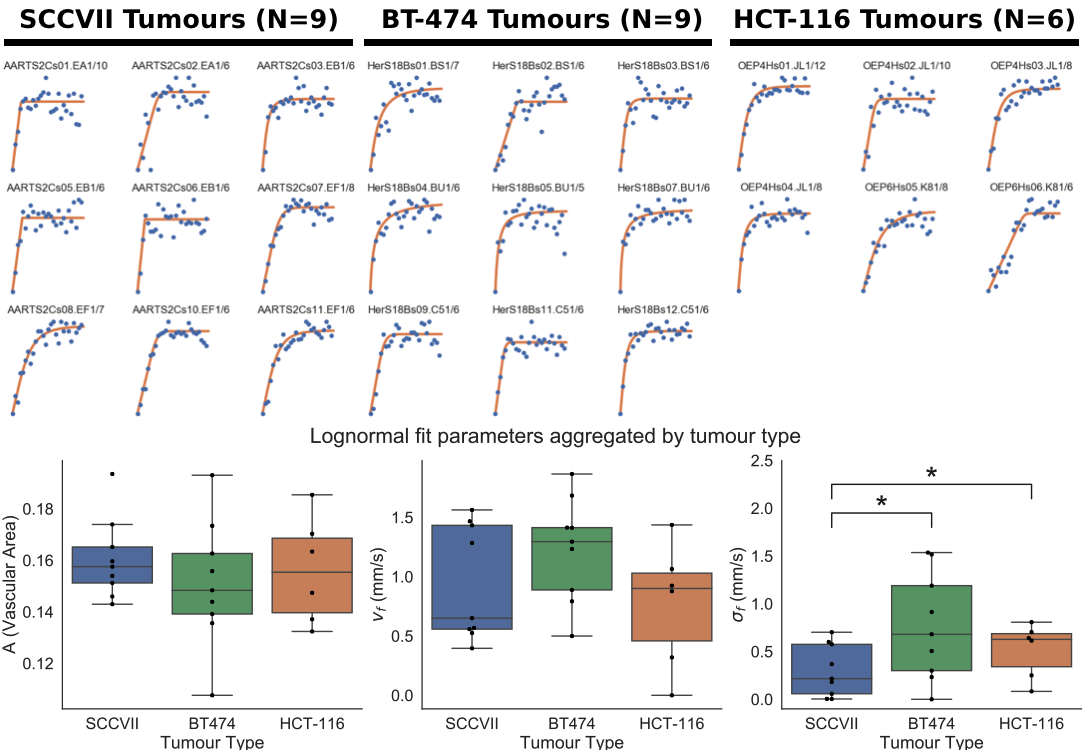
\includegraphics[width=\textwidth]{oemri_thesis2/oemri_thesis2-images/lognormalFittingAgg_CHB.png} % requires the graphicx package
   \caption{Top: Individual fits to the oxygen response curve for each animal and tumour type.
   Bottom: Box plots showing the median value and quartiles for $A$, $v_f$m and $\sigma_f$ across the three tumour models.}
   \label{fig:lognormal_CHB}
\end{figure}
%%%%%%%%%%%%%%%%% ############ END section about fitting ############ 

%%%%%%%%%%%%%%%%% ############ BEGIN *histo validation* section from paper 1 ############ 

\subsection{dOE-MRI maps correspond to matched histology sections}
\label{sec:histoSections}
Tumour tissue cryosections obtained to match MR imaging slices were stained for vasculature (CD31) and regions of pimonidazole-labeled hypoxia and are compared side-by-side; Figures~\ref{fig_sccvii} and~\ref{fig_hct116} provide five examples for each of SCCVII and HCT-116 tumour models for detailed review.
Generally, in corresponding dOE-MRI maps for both tumour models O$_2$-positive voxels align with the most oxygenated regions of histology sections, where pimonidazole labeling is absent, however many areas of mismatch are also observed. 
More consistent is that O$_2$-positive voxels do not typically correspond to tissues identified as hypoxic in the histology sections (i.e. labeled with pimonidazole).
In general, the more necrotic HCT-116 tumours have fewer oxygenated (O$_2$-positive) regions and significantly more hypoxic (O$_2$-negative) regions in the dOE-MRI maps, compared to the SCCVII tumours that have no necrosis. 
Pimonidazole labeling is heterogeneously dispersed within regions of viable tissue containing tumour blood vessels for both SCCVII tumours, Figure~\ref{fig_sccvii}, and HCT-116 tumours, which typically have greater amounts of necrosis, Figure~\ref{fig_hct116}.
Figure~\ref{histo_correlations} shows the fraction of negative dOE-MRI voxels correlated with the histological hypoxic fraction. 
For SCCVII tumours (n=9) there was an excellent correlation, with Pearson's r = 0.91 (\textit{p}=0.0016). 
However the correlation in the HCT-116 tumours (n=6) was poor, with r=0.13 (\textit{p}=0.81). 

\begin{figure}[htbp]
   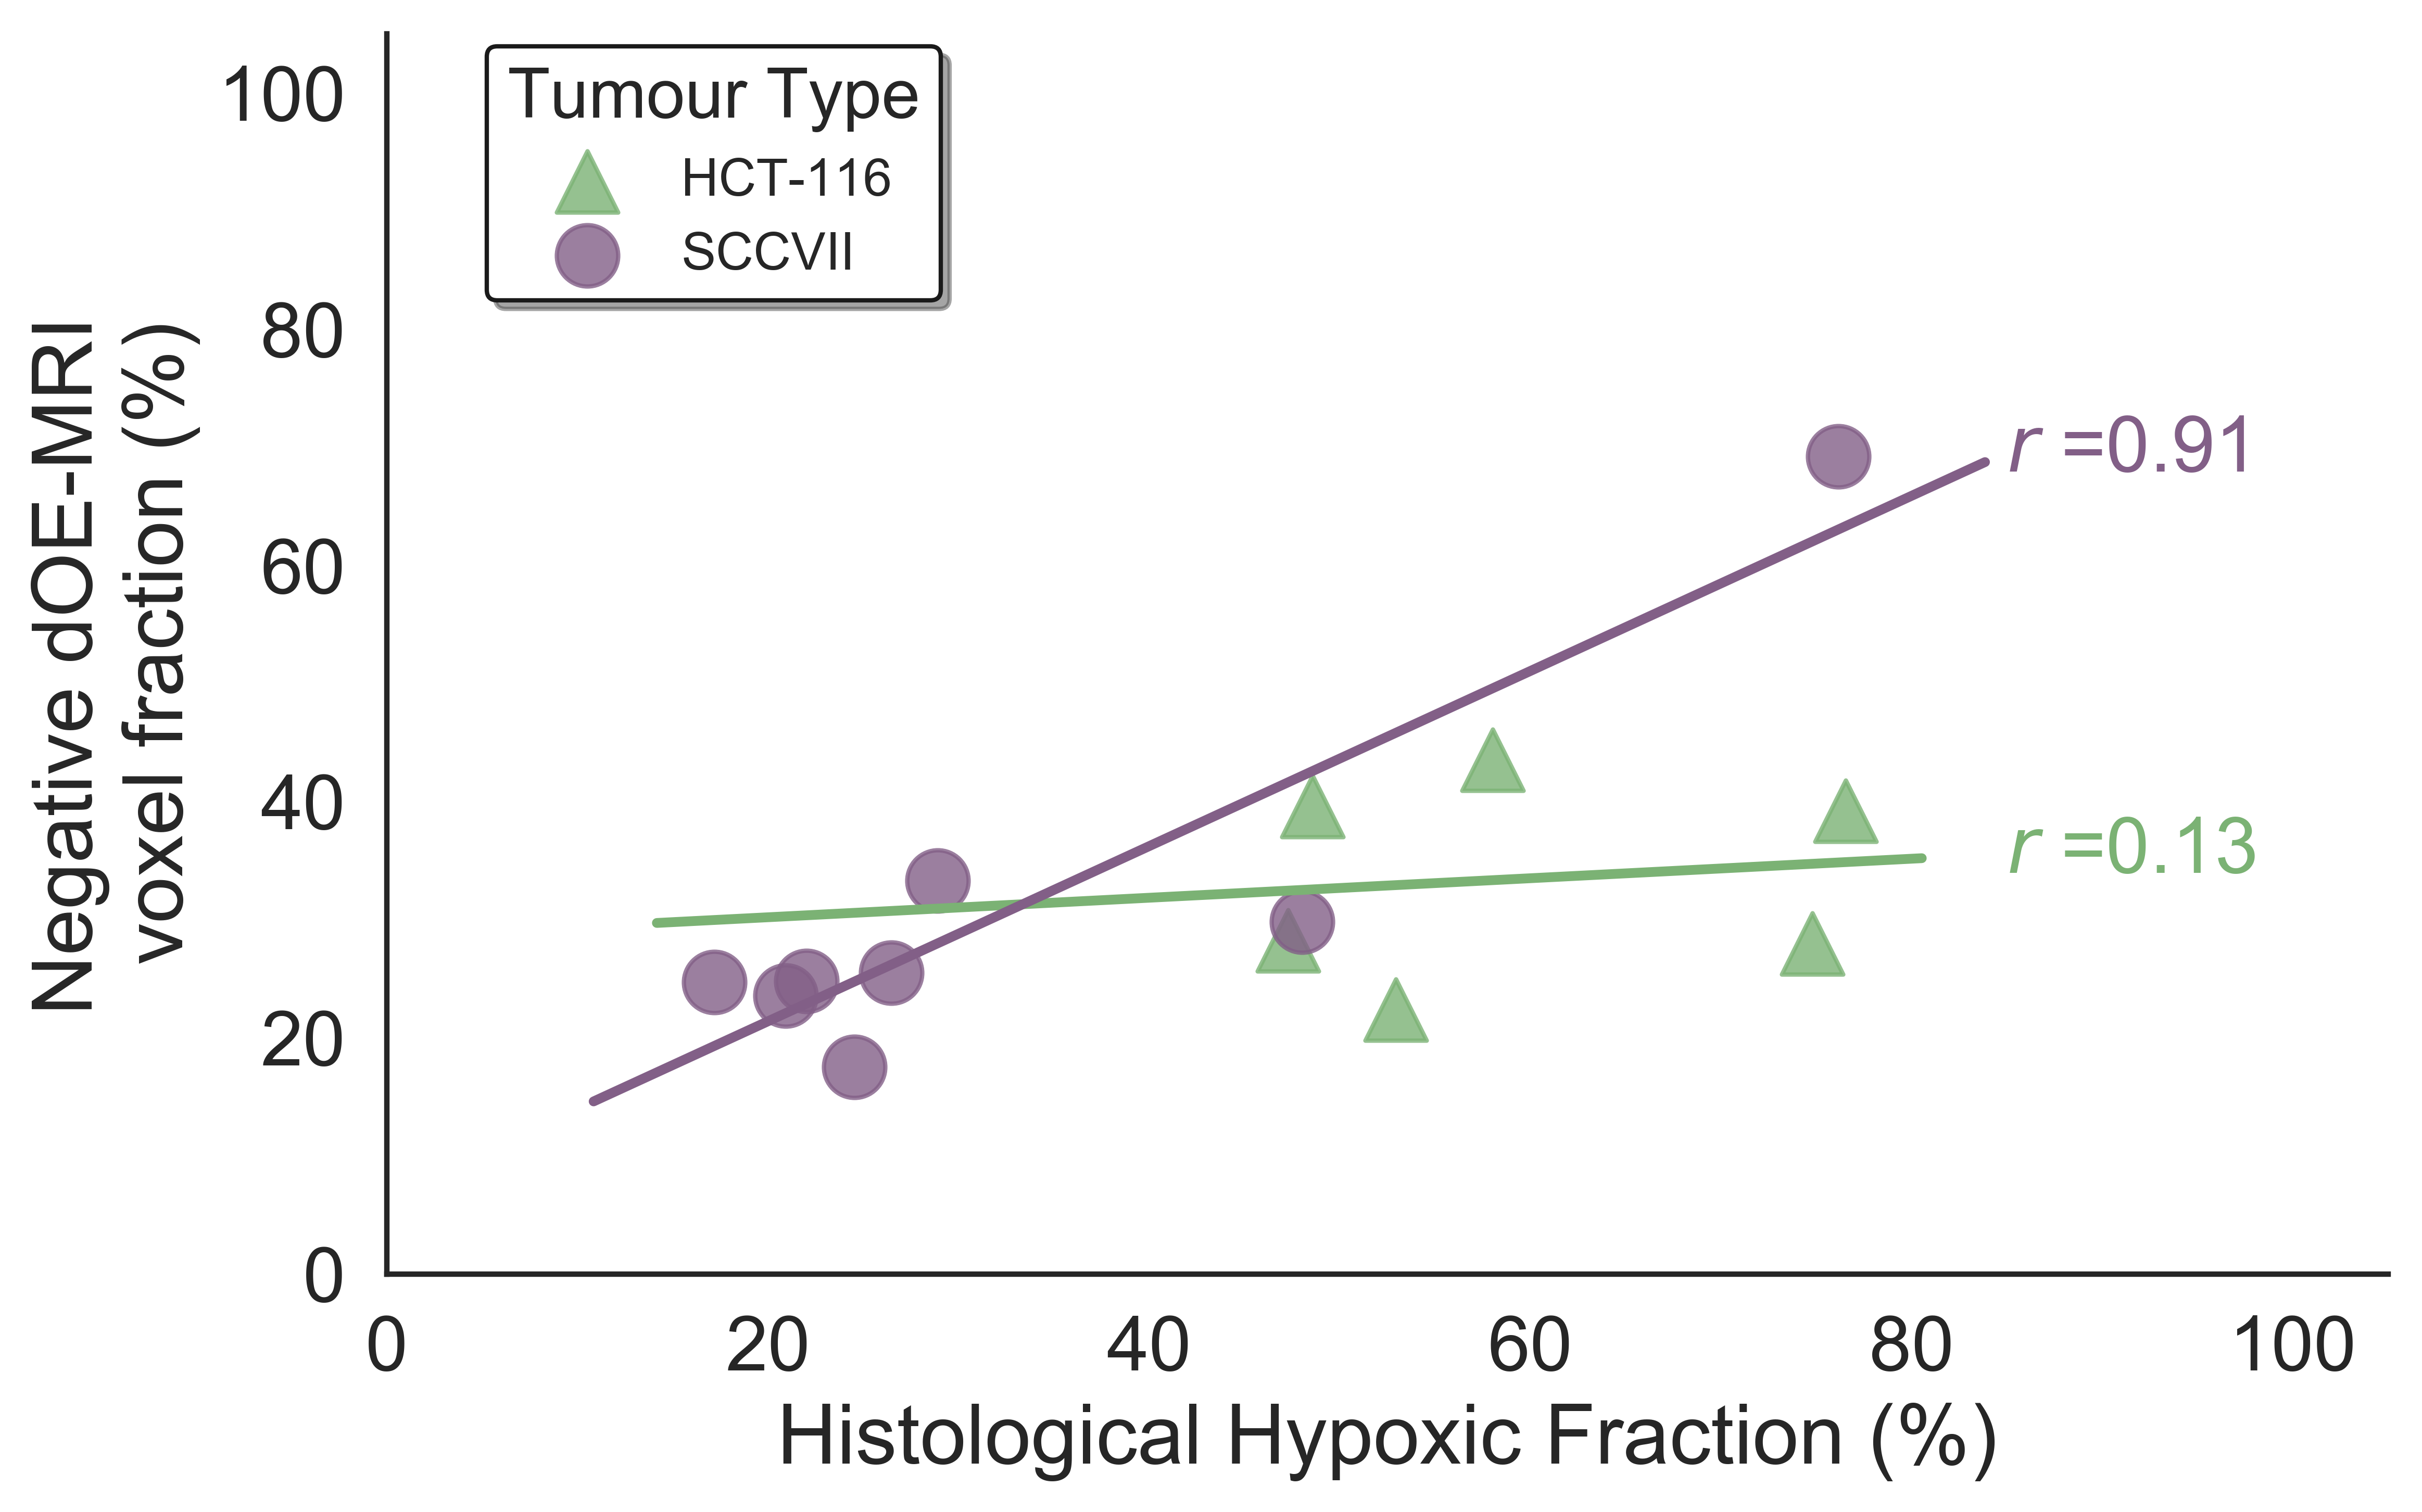
\includegraphics[width=\textwidth]{oemri_thesis1/oemri_thesis1-images/histocorrel2.png} % requires the graphicx package % note for Firas: I changed the aspect ratio of this figure slightly
   \caption{The proportion of negative dOE-MRI voxels is plotted against the histological hypoxic fractions with Pearson's r = 0.91 for SCCVII tumours and r = 0.13 for HCT-116 tumours.
   \label{histo_correlations}}
\end{figure}

\begin{figure}[htbp]
   \centering
   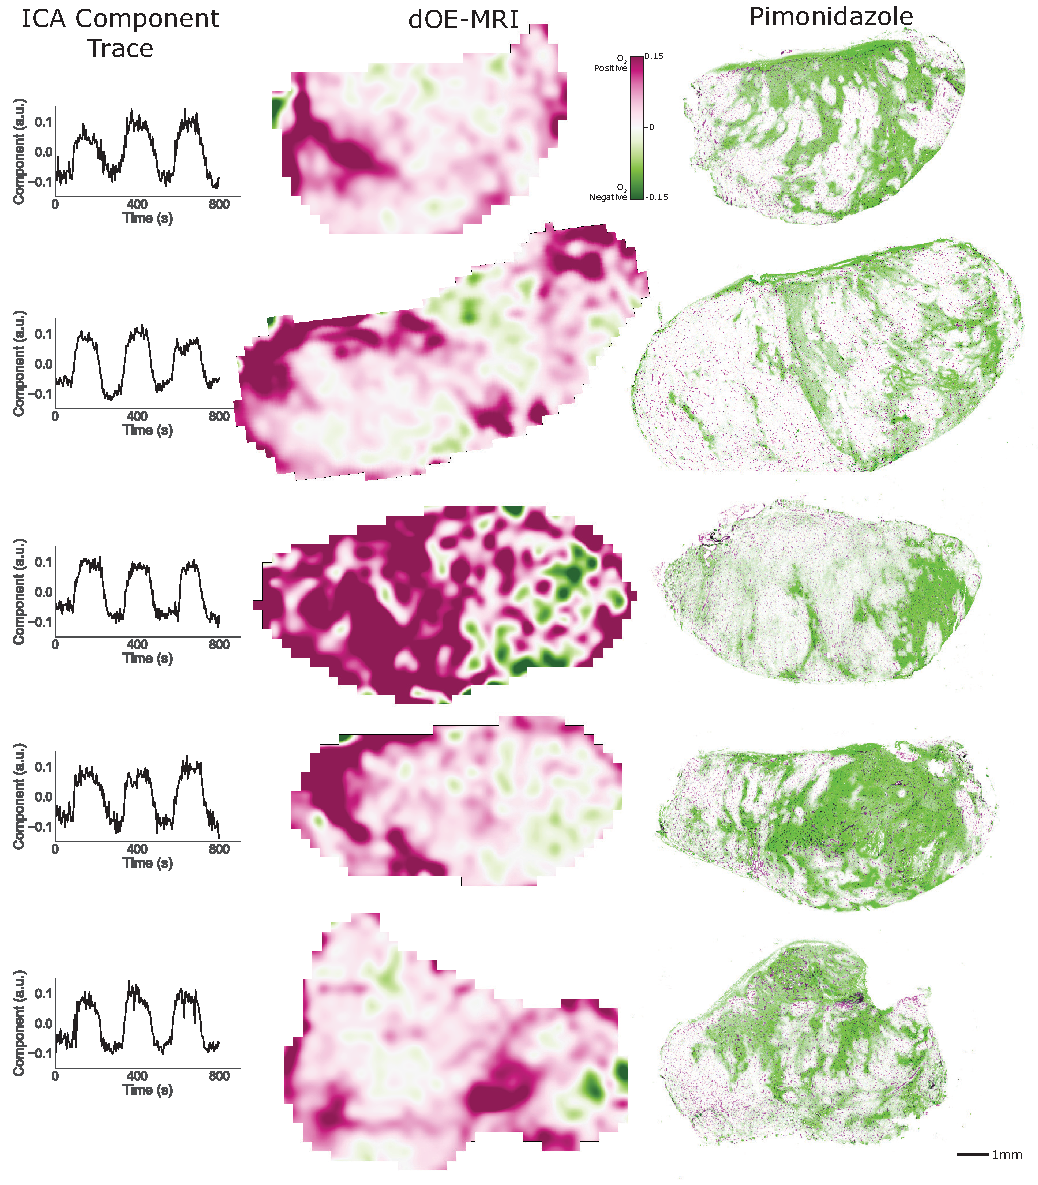
\includegraphics[width=0.9\textwidth]{oemri_thesis1/oemri_thesis1-images/fig6_sccvii.pdf} % requires the graphicx package
   \caption{SCCVII murine tumours with slice-matched histological images depicting pimonidazole-labeled hypoxia (green) and CD31-stained vasculature (purple) are shown next to the dOE-MRI parameter maps similarly colored with O$_2$-positive (purple) and O$_2$-negative (green) areas. Corresponding ICA extracted components are also shown.
   \label{fig_sccvii}}
\end{figure}
\begin{figure}[htbp]
   \centering
   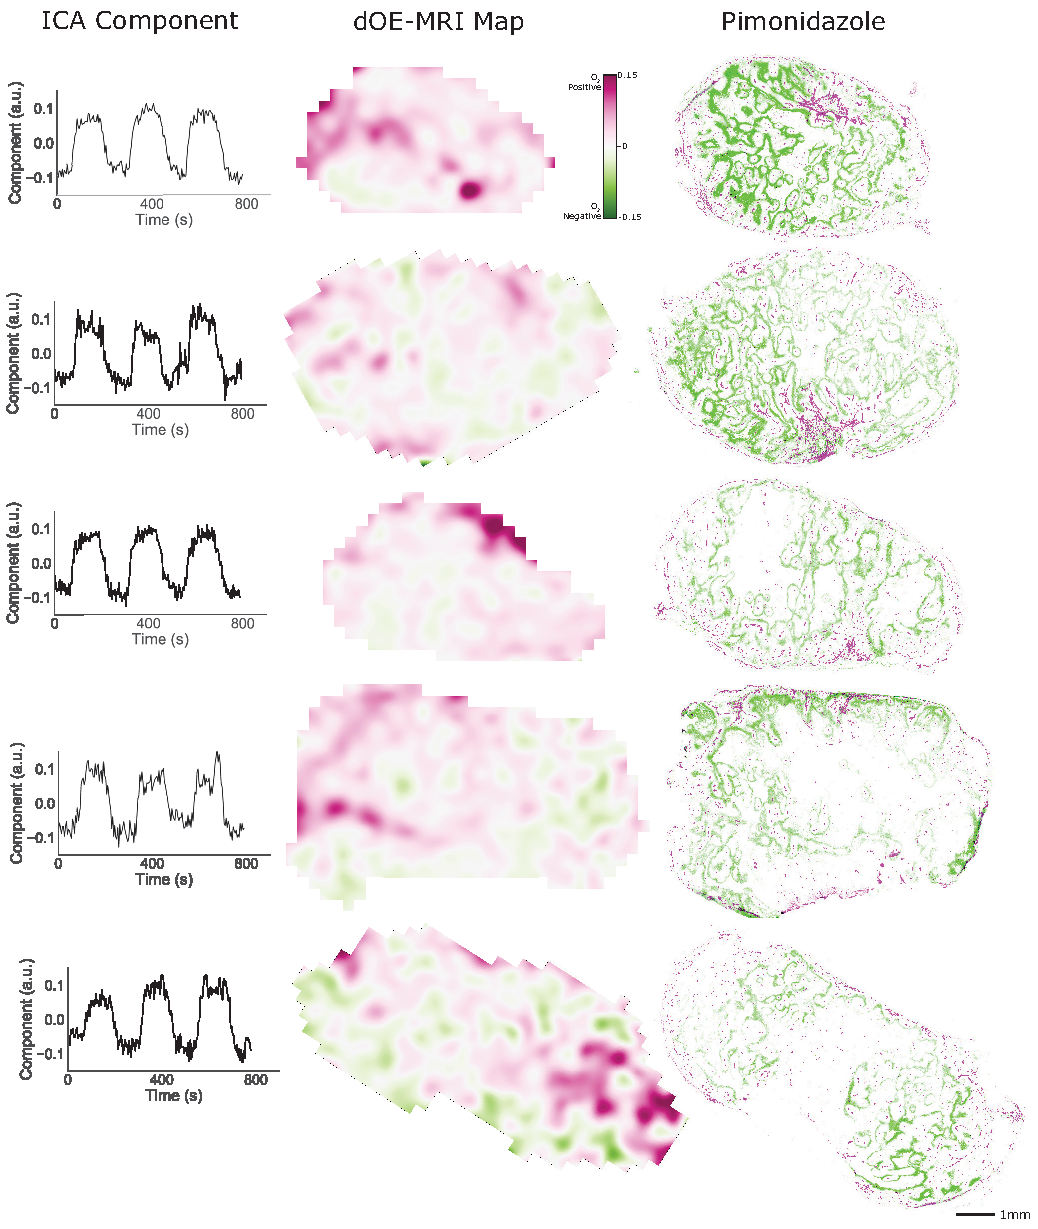
\includegraphics[width=0.9\textwidth]{oemri_thesis1/oemri_thesis1-images/fig7_hct116.pdf} % requires the graphicx package
   \caption{HCT-116 human colorectal xenografts with slice-matched histological images depicting pimonidazole-labeled hypoxia (green) and CD31-stained vasculature (purple) are shown next to the dOE-MRI parameter maps similarly colored with O$_2$-positive (purple) and O$_2$-negative (green) areas. Corresponding ICA extracted components are also shown.
   \label{fig_hct116}}
\end{figure}

%%%%%%%%%%%%%%%%% ############ END *histo validation* section from paper 1########### 

% ======================================================================
\section{Discussion}
% ======================================================================

The improved sensitivity of our dOE-MRI technique results in broader applicability of dOE-MRI, as we found that an oxygen-enhancing component was extracted successfully in all imaged animals across a range of tumour models and environments (Figure~\ref{versatile}).
In this study we also modelled the oxygen response curves in the tumour vasculature by deploying models developed in DCE-US and adapting them for dOE-MRI.
Fitting equation~\ref{lognormalFitEquation} to the oxygen response curves results in three physiologically relevant parameters.
Unsurprisingly, the vascular area $A$ and the mean velocity $v_f$ do not appear to be vary between the three tumour models studied(Figure~\ref{fig:lognormal_CHB}).
The third parameter $\sigma_f$ is the standard deviation of the velocity distribution and is related to the structural organization and morphology of the vascular network~{\cite{Hudson:2009jv}.
Thus, we hypothesized that the oxygen response curves and in particular, $\sigma_f$ may capture information about the vascular organization in different tumour models.
The SCCVII tumour is a very aggressive and fast growing tumour~\todo{would be nice to have a ref here}, which implies a chaotic vascular network with a low degree of fractality (propensity to branch in a fractal pattern with large arteries branching to smaller arterioles, leading to extremely small capillaries).
This behaviour would result in a narrow range of vessel sizes and velocity profiles in our lognormal velocity profile,  and manifests in a low $\sigma_f$ value for SCCVII tumours relative to the other tumour lines.
While only $\sigma_f$ appears to be useful in delineating tumour models, $v_f$ and $A$ may be useful metrics to quantify the oxygen response curves of tumours after drug interventions. 
  
A limitation of OE-MRI is the difficulty in interpreting areas that do not show a reduction in T$_1$ as they may be either dead tissues that are \textit{unperfused and not oxygenated} or living, viable tissues that are \textit{perfused but not oxygenated} due to poor oxygen content of the supplying vessels. 
The latter population are of greater interest to the oncology community as it is these hypoxic but viable cells that have significant influence on treatment outcomes~\cite{Horsman:2016go}. 
The dOE-MRI technique presented here successfully correlates tumour oxygenation dOE-MRI and histology measures in SCCVII tumours but, despite improvements to sensitivity, a similar quantitative comparison in the HCT-116 tumour line showed poorer association (Fig.~\ref{histo_correlations}). 
This is likely attributable to the much higher amounts of necrosis typical of the HCT-116 model relative to SCCVII (Figs.~\ref{fig_sccvii} and \ref{fig_hct116}).
Mitigations to this limitation have been explored elsewhere and generally require a perfusion mask or $T_2^*$ - either technique can be added to the OE-MRI method proposed here to exclude necrosis and further improve sensitivity of the technique.

Application of existing OE-MRI techniques across a range of tumour models with varying perfusion characteristics has yielded mixed success without masking for perfused tissue.
For instance, O'Connor reported that in the highly perfused 786-0-R tumour lines, 85-96\% of all imaged tumour voxels were deemed to be oxygen-enhancing~\cite{OConnor:2016ee}.
In those tumours, there was a good correlation between histological hypoxic fraction and oxygen refractory voxels.
However, in the more weakly perfused SW620 tumours where only 76\% of the voxels are oxygen-enhancing, there were no significant correlations with the histological hypoxic fraction.
These issues were resolved by combining OE-MRI with DCE-MRI as a perfusion mask to select only perfused voxels for oxygenation assessment, thereby distinguishing between the viable hypoxic environment and necrotic dead tissues and improving the specificity and sensitivity of OE-MRI data. Using an IAUGC$_{60}$ map from DCE-MRI as a mask to obtain Oxy-R fractions O'Connor et al. showed good correlation with the histological hypoxic fraction~\cite{OConnor:2016ee}.
In more recent work, Little et al. showed oxygen enhancement in tumours with a histological hypoxic fraction as high as 43\%~\cite{Little:2018iu} and this translated very well to a study of six renal cell carcinoma patients.
Linnik et al. reported excellent correlation between percentage of ``negative AUC$_{OE}$'' ($O_2$-negative) voxels and percentage of hypoxic areas in the highly vascular preclinical U87MG tumour xenografts~\cite{Linnik:2013hf}.
A second approach for differentiating between viable but hypoxic regions and unperfused dead tissues, is to combine OE-MRI with $T_2^*$W acquisition and the BOLD effect to classify regions~\cite{Little:2018iu,Zhao:2015ez,White:2016fz,Burrell:2013je,Yang:2018vo} that show both effects. 
Excess oxygen in the blood will induce changes in Hb saturation, which alter the T2* resulting in a robust measure of areas with functioning vasculature. 
Conceivably, the saved acquisition time achieved with under-sampling T$_1$W dOE-MRI suggests that $T_2^*$W images could also be acquired to concurrently assess the blood oxygen level dependent (BOLD) response. 

Within the relatively short 14-minute imaging time, both the HCT-116 and SCCVII tumours show only minor changes in the oxygenation maps between cycles (Figure~\ref{fig_correlation}).
In longer imaging sessions, or during administration of an intervention, these same tumours may exhibit varying oxygenation patterns between cycles.
Periods of oxygen-starvation and re-oxygenation in tumours have been termed intermittent hypoxia and can arise due to temporary vessel occlusions~\cite{Dewhirst:2009de,Bayer:2011js}.
Recent work on measuring intermittent hypoxia in patients using R$_2^*$~\cite{Panek:2017ge} shows that interest in this phenomenon continues but the importance of intermittent hypoxia in tumours is unclear largely due to poor availability of techniques to measure it in the clinic~\cite{Michiels:2016hv}.
The relatively short imaging time for dOE-MRI makes assessing temporal oxygenation changes possible within a timescale on the order of minutes by comparing correlation maps generated from sequential cycles.

Typically, histological validation of MR data is done by collapsing rich histology data into a single metric, such as a hypoxic fraction, with whole-tumour or single-slice average comparisons.
While this is sometimes a useful validation approach, it may not reflect the highly heterogeneous patterns of hypoxia that are known to vary spatially and temporally, even within the same tumour, as well as between tumour types as highlighted in Figures~\ref{histo_correlations}-\ref{fig_hct116}. 
Further complications are encountered with respect to validation of tools to assess hypoxia considering that hypoxia is not simply a binary metric. Instead, tumour oxygenation exists as a spectrum beginning with some tissues that may be normoxic, at levels similar to neighbouring normal tissues of origin, and can continue decreasing through levels of hypoxia to near anoxia where cells are still viable but are no longer able to proliferate.
Eventually cells die in the absence of oxygen, and when this occurs in large numbers there can be significant regions of necrosis in solid tumours. 
A range of oxygenation levels are likely to be present in the highly heterogeneous microenvironments of all solid tumours, but what is of interest to the oncology community is \emph{clinically relevant} hypoxia~\cite{Horsman:2012kw}.
This refers to measurable tumour oxygenation levels that are biomarkers of physiologically meaningful phenomena, including patient prognosis or tumour sensitivity to treatments, such as immunotherapy or radiotherapy. The relevant oxygenation status for any biomarker of interest may include levels spanning from moderate to severely hypoxic. 
Pimonidazole has been demonstrated as a clinically relevant marker of hypoxia, but poor or inconsistent correlation with pimonidazole, as we have seen in our imaged tumours, does not exclude other measures of tumour oxygenation from potential utility.

Measurable pimonidazole-adduct formation occurs when the O$_2$ tension in the vicinity drops below 10 mmHg~\cite{Gross:1995wq} but in dOE-MRI, O$_2$-positive voxels are extracted as excess oxygen dissolves in the plasma and interstitial tissue fluid to decrease T$_1$.
Voxels where T$_1$ has significantly increased has previously been correlated to poorly perfused regions and likely corresponds to hypoxic regions where the excess oxygen is picked up by deoxyhemoglobin molecules~\cite{Linnik:2013hf,Burrell:2013je,Remmele:2012df}.
The exact mechanism for a T$_1$ increase as a result of oxygen inhalation has not yet been confirmed~\cite{Zhao:2015ez,Linnik:2013hf}, however, based on careful work of Silvennonin et al., characterizing behavior of T$_1$ in fresh bovine blood~\cite{Silvennoinen:2003gn}, we speculate the corresponding T$_1$W signal decrease may arise due to the conversion of deoxyhemoglobin to hemoglobin in the perfused vessels of hypoxic regions .
O$_2$-positive regions in dOE-MRI maps are generally in good agreement with well perfused areas of histology images for both HCT-116 and SCCVII tumours, as shown in Figures~\ref{fig_sccvii} and~\ref{fig_hct116}.
Voxels exhibiting signal reduction with the O$_2$ stimulus in dOE-MRI maps (O$_2$-negative, green) typically correspond with histology (pimonidazole, green) but not all pimonidazole-labeled regions appear as O$_2$-negative voxels.
Similarly, CD31-stained tumour regions are not exclusively O$_2$-positive in the dOE-MRI maps because not all tumour vessels are perfused.
In fact many perfused blood vessels are only intermittently perfused and consequently, the measurement of hypoxia is time-sensitive.
Mismatches between dOE-MRI and histology may be attributed in part to the different sensitivities and detection thresholds for measuring hypoxia and oxygenation in the dOE-MRI and histology-based modalities, as well as potential mismatch between the timing of pimonidazole-labeling and dOE-MRI data acquisition. 

%\subsection{random snippets}
%O$_2$ positive or O$_2$-negative fractions are immune to this phenomenon, information about the level of response can be retained simply by applying the scaling factor when comparing scans at different temporal resolutions
% ======================================================================
\section{Conclusions}
% ======================================================================

In this chapter, we have validated the dOE-MRI technique by comparing oxygenation maps with pimonidazole stained histology images. 
The versatility of the technique was apparent due to its applicability in multiple tumour models; though, the presence of large necrotic areas in tumours poses some challenges when comparing oxygenation status with pimonidazole staining.
We have also shown that the lognormal velocity profile model from DCE-US is applicable to oxygen response curves obtained from ICA and dOE-MRI and the parameter $\sigma_f$ is useful in quantifying the vascular morphology of tumours.
dOE-MRI assesses tumour oxygenation fairly reliably \emph{in vivo} and the next application is to see whether the technique is sensitive to oxygenation changes brought on by chemotherapies.
% ======================================================================
\section{Acknowledgments}
% ======================================================================

This work was supported by NSERC and CIHR.

% ======================================================================
 %\section{References}
% ======================================================================
%\bibliography{oemri2}

%\bibliographystyle{vancouver-authoryear}

%\end{document}